\documentclass[12pt,twoside]{article}
\usepackage{amsmath, amssymb}
\usepackage{amsmath}
\usepackage{fancyhdr,parskip}
\usepackage[active]{srcltx}
\usepackage{amssymb}
\usepackage{amscd}
\usepackage{makeidx}
\usepackage{amsthm}
\usepackage{algorithm}
\usepackage{algpseudocode}
\usepackage{fancyhdr}
\usepackage{graphics}
\usepackage{amsmath, amssymb}
\usepackage{amsmath}
\usepackage[active]{srcltx}
\usepackage{amssymb}
\usepackage{amscd}
\usepackage{makeidx}
\usepackage[dvips]{graphicx}
\usepackage{longtable}
\usepackage{tabularx}
\usepackage[table,xcdraw]{xcolor}
\usepackage{color}
\usepackage[hidelinks]{hyperref}
\usepackage[backend=biber,style=apa]{biblatex}
\usepackage{longtable}
\usepackage{tabularx}
\usepackage[table,xcdraw]{xcolor}
\usepackage{color}
\usepackage[hidelinks]{hyperref}
\usepackage{multirow}
\usepackage{algorithm}
\usepackage{algpseudocode}
\usepackage{fancyhdr,graphicx,amsmath,amssymb}
\renewcommand{\algorithmicrequire}{\textbf{Input:}}
\renewcommand{\algorithmicensure}{\textbf{Output:}}
\renewcommand{\tablename}{Tabla}
\renewcommand{\figurename}{Figura}
\renewcommand{\baselinestretch}{1}
\setcounter{page}{1}
\setlength{\textheight}{21.6cm}
\setlength{\textwidth}{14cm}
\setlength{\oddsidemargin}{1cm}
\setlength{\evensidemargin}{1cm}
\pagestyle{myheadings}
\thispagestyle{empty}
\markboth{\small{Pr\'actica Extra. Luis Francisco Renteria Cedillo, Denzel Omar Vazquez Perez.}}{\small{.}}
\date{}
\begin{document}
    \begin{figure}[h]
    \vspace{-3cm} \hspace{-2cm} \setlength{\unitlength}{1mm}
    \begin{picture}(15,25)(-10,0)
    
\includegraphics[width=16.5cm,height=2.8cm]{imagenes/titulo.png}
    \end{picture}
    \end{figure}
    \vspace{0cm}
    \centerline{\bf An\'alisis de Algoritmos, Sem: 2022-2, 3CV11, Pr\'actica Extra, 07 de junio de 2022}
    \centerline{}
    \begin{center}
    \Large{\textsc{Pr\'actica Extra: Algoritmo de Dijkstra}}
    \end{center}
    \centerline{}
    \centerline{\bf {Luis Francisco Renteria Cedillo, Denzel Omar Vazquez Perez.}}
    \centerline{}
    \centerline{$lrenteriac1400@alumno.ipn.mx, dvazquezp1600@alumno.ipn.mx$}
    \newtheorem{Theorem}{\quad Theorem}[section]
    \newtheorem{Definition}[Theorem]{\quad Definition}
    \newtheorem{Corollary}[Theorem]{\quad Corollary}
    \newtheorem{Lemma}[Theorem]{\quad Lemma}
    \newtheorem{Example}[Theorem]{\quad Example}
    \bigskip

\textbf{Resumen:} En el presente documento se muestra el an\'alisis {\it a Priori} y {\it a Posteriori} a el algoritmo de Dijkstra para determinar su complejidad temporal a partir de su implementaci\'on en el lenguaje de programaci\'on C con matrices de adyacencia.

{\bf Palabras Clave:} Dijkstra, Matriz, Greedy, Soluci\'on optima, Lenguaje C.

\section{Introducci\'on}
Siempre ha habido problemas donde se requiere encontrar el camino más corto entre un conjunto de puntos incluso en la informática. Hay muchos m\'as ejemplos y comunes, desde la navegaci\'on por sat\'elite hasta el enrutamiento de paquetes de Internet; incluso encontrar la longitud de cable m\'as corta para conectar los pines en una placa de circuito.\\

Al tener mucha recurrencia este tipo de problemas surgen algunos algoritmos est\'andar que se pueden utilizar para encontrar una soluci\'on, uno de ellos se conoce como algoritmo de Dijkstra, diseñado por el f\'isico holand\'es Edsger Dijkstra en 1956, cuando pens\'o en c\'omo podr\'ia calcular la ruta m\'as corta de Rotterdam a Groningen.\\
Este algoritmo tiene bastas aplicaciones para resolver una amplia variedad de problemas complejos, ya que esta escrito en el contexto de grafos ponderados, por lo que todo el lenguaje lo refleja pues esta compuesto de v\'ertices y aristas. 
Por tanto, este algoritmo funcionar\'a en cualquier cosa que pueda abstraerse a una serie de vértices que est\'en conectados y tienen valores adjuntos a esas conexiones.\\

As\'i el algoritmo funciona bien para la b\'usqueda de rutas para un conjunto completo de vértices pero, cuando se usa para buscar la ruta más corta a un objetivo espec\'ifico, puede ser ineficiente y no se podrían obtener soluciones al problema.

\section{Conceptos B\'asicos}
    \subsection{Matrices de adyacencia}
        Una matriz de adyacencia representa un grafo con una matriz $nxn$ donde $n$ es $|V|$. As\'i, si $M=[E(i,j)]$ donde cada elemento $E(i,j)$ contiene los atributos de la arista. Si las aristas no tienen un costo, el grafo se puede representar mediante una matriz booleana para ahorrar espacio en la memoria v\'ease Figura 1.
        \begin{figure}[H]
            \centering
            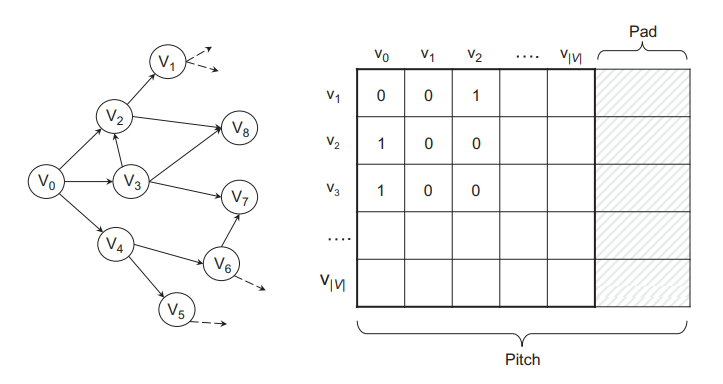
\includegraphics[height=7cm]{imagenes/c1.png}
            \caption{Matrices de adyacencia}
        \end{figure}
        Los mas comunes algoritmos que usan esta representación son la ruta más corta de todos los pares, donde si el gráfico es ponderado, cada valor de $E(i,j)$ se define de la siguiente manera:\\
        $$M[i,j]= \left\{ \begin{array}{lcc}
            0 &   si  & i=j\\
            \\ w(i,j) &  si & i=j~y~(i,j)\in E\\
            \\ \infty &  si & i\neq j~y~(i,j)\notin E
            \end{array}
            \right.$$
        \\
    \subsection{Algoritmos Greedy}
        Los algoritmos Greedy emplean un procedimiento de resoluci\'on de problemas para construir progresivamente soluciones candidadtas \'optimas, para aproximarse al \'optimo global, obteniendo mejores soluciones \'optimas localmente en cada etapa. As\'i con esta estrategia de soluci\'on de problemas no se puede producir una solución óptima global, pero si buenas soluciones \'optimas localmente en un tiempo razonable y con menos esfuerzo computacional, v\'ease {\bf Algorithm 1} para ver la estructura de la implementaci\'on general de la estrategia.
        \begin{algorithm}[H]
        \caption{FuntionGreedy(set C) }
            \begin{algorithmic}[1]
                \State S=$\emptyset$
                \While{$\neg$isSolution(S) \&\& C$\neq \emptyset$}
                    \State x=select$\_$best$\_$option(C)
                    \State C=C-\{x\}
                    \If{isOptimum(S$\cup$\{x\}}
                        \State S=S$\cup$\{x\}
                    \EndIf
                \EndWhile
                \If{isSolution(S$\cup$\{x\}}
                    \State return S
                \EndIf
            \end{algorithmic}
        \end{algorithm}
    \subsection{Algoritmo de Dijkstra}
        El algoritmo de Dijkstra es el m\'etodo elegido para encontrar las rutas más cortas en un grafo ponderado por aristas y/o vértices. Dado un v\'ertice de inicio particular, encuentra la ruta mas corta a cualquier otro v\'ertice en el grafo, incluido el v\'ertice destino, v\'ease Figura 2.
        \begin{figure}[H]
            \centering
            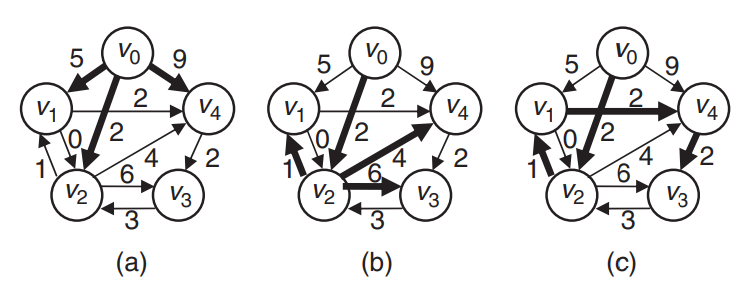
\includegraphics[height=6cm]{imagenes/c2.png}
            \caption{Ejemplo del algoritmo de Dijkstra}
        \end{figure}
    \subsection{Pseudoc\'odigo del algoritmo de Dijkstra}
        El pseudoc\'odigo del {\bf Algorithm 2} muestra el algoritmo de Dijkstra que a partir de un grafo G, haciendo uso de matrices de adyacencia y al inicializar los arreglo S, D y P, repetidamente realiza la diferencia entre los conjuntos de V y S, para tomar el menor peso w de V-S e insertando este en S, luego se comparan los v\'ertices que est\'an en V-S, pasando por cada uno de estos para para encontrar el valor m\'inino de D[v] y D[w] G[w,v], para su inserci\'on en de w en P[v], terminando si V-S en $\emptyset$.
        \begin{algorithm}[H]
        \caption{ Dijkstra(G:Graph, initial:node,V:V\'ertex)}
            \begin{algorithmic}[1]
            \State Inicializar(G,V)
            \State S=$\{0,...,|V|-1\}$
            \State D=$\{0,...,|V|-1\}$
            \State P=$\{0,...,|V|-1\}$
            \State insert(initial,S)
            \For {v$\in$V, v$\neq$initial }
                \State D[v]= G[initial,v]
                \State P[v]=initial
            \EndFor
            \While{V-S$\neq \emptyset$}
                \State getMin(w$\in$V-S)
                \State S=S$\cup$\{w\}
                \For{v$\in$V-S}
                    \State D[v]=min(D[v], D[w]+G[w,v])
                    \If{min(D[v], D[w]+G[w,v])=D[w]+G[w,v]}
                        \State P[v]=w
                    \EndIf
                \EndFor
            \EndWhile
            \end{algorithmic}
        \end{algorithm}

\section{Experimentaci\'on y Resultados}
    \subsection{An\'alisis a Priori}
    Dada la implementaci\'on del {\bf Algorithm 2} en el lenguaje de programaci\'on C se tiene la siguiente codificaci\'on. Donde a partir de un grafo se genera una matriz adyacente para su posterior ejecuci\'on, entonces dado cada bloque de sentencia del algoritmo, se muestra la obtenci\'on del orden de complejidad para el peor caso de este por medio de un an\'alisis de segmentos de c\'odigo, véase Figura 3, donde se concluye que $T(n)\in\Theta(n^{2})$
    \begin{figure}[H]
        \centering
        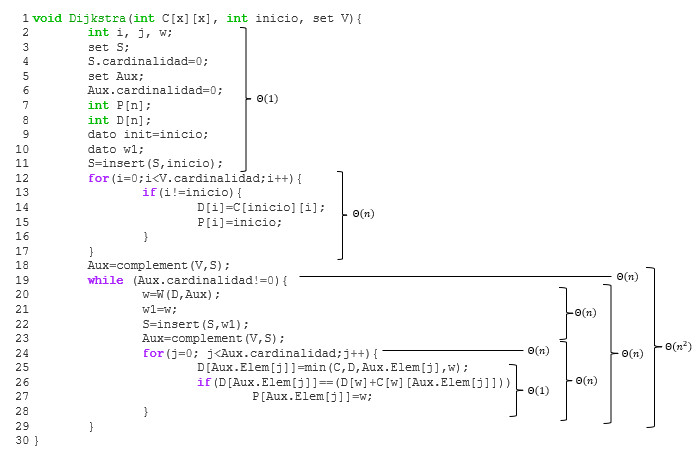
\includegraphics[height=9cm]{imagenes/AD.png}
        \caption{Implementaci\'on del algoritmo de Dijkstra en lenguaje C}
    \end{figure}
    As\'i el algoritmo mantienen invariante el $Aux=V-S$ al comienzo de cada iteraci\'on del bucle while de las lineas 19-30. En la linea 11 se inicializa el arreglo S para contenga el v\'ertice de partida hasta contener todos los v\'ertices de V, desde insert(initial,S) en ese momento se cumple la condici\'on de la linea 19 si V-S$\neq\emptyset$.\\
    
    Por lo que cada vez que pasa por el bucle while, en la linea 20 se extrae el v\'ertice con la distancia menor cumpliendo que D[v]$\in$Aux, as\'i se coloca este en el arreglo S, obteniendo de nueva cuenta $Aux=V-S$ para pasar por cada uno de los elementos del conjunto Aux, para obtener la m\'inima distancia para cada $v\in Aux$ tal que $D[v]=min(D[v], D[w]+G[w,v])$, donde si $D[v]=D[w]+G[w,v]$ se inserta el v\'ertice w en el arreglo P. Por tanto hay que observar que el algoritmo nunca inserta v\'ertices de V despu\'es de la linea 18, y que cada v\'ertice se extrae de V y se inserta en S exactamente una vez de modo que el ciclo while de la lineas 19-30 itera exactamente $|V|$ veces, donde $n=|V|$.\\
    
    Ante esto se puede decir que el algoritmo de Dijkstra al siempre elegir el v\'ertice con menor costo en V-S para agregarlo al conjunto S, se puede afirmar que este usa una estrategia Greevy.
    
    \subsection{An\'alisis a Posteriori}
    Al ejecutar la funci\'on con el nombre {\it Dijkstra }, con la asignaci\'on de valores de entrada por una matriz de adyacencia C, un nodo inicial y el conjunto de todos los v\'ertices, se muestran los siguientes ejemplos de la ejecuci\'on, donde los arreglo S representa la soluci\'on al problema, el arreglo D las distancias desde el nodo inicial a cada uno de los nodos y el arreglo P la contrucci\'on de los caminos correspondientes.\\
    El primer grafo implementado tiene $|$V$|$=4 entonces, si se escoge como variable inicial=0 se tiene los siguientes resultados, v\'ease Figura 4.
    \begin{figure}[H]
        \centering
        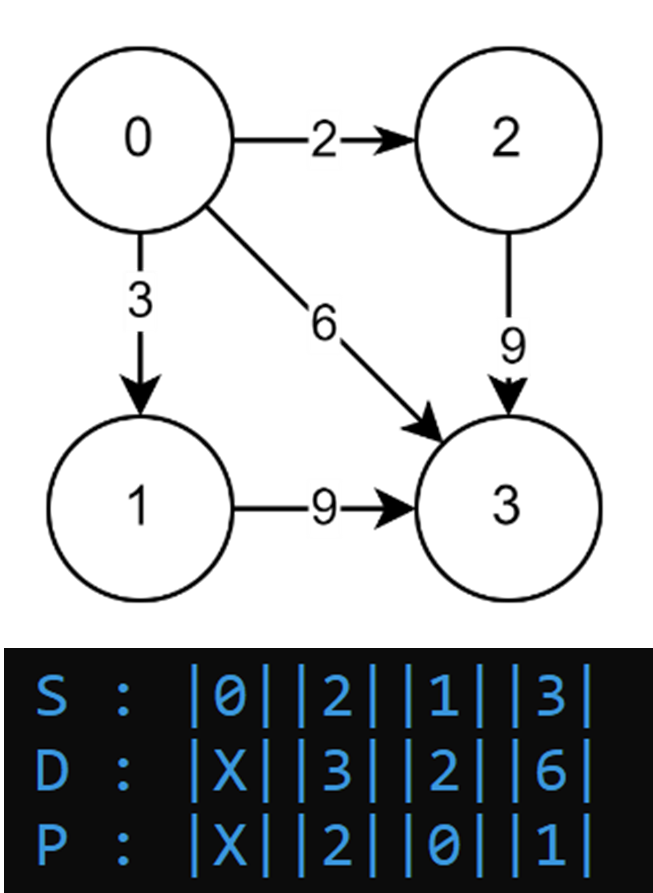
\includegraphics[width=4cm]{imagenes/Imagen1.png}
        \caption{Ejemplo 1 del algoritmo de Dijkstra}
    \end{figure}
    El segundo grafo implementado tiene $|$V$|$=5 entonces, si se escoge como variable inicial=2 se tiene los siguientes resultados, v\'ease Figura 5.
    \begin{figure}[H]
        \centering
        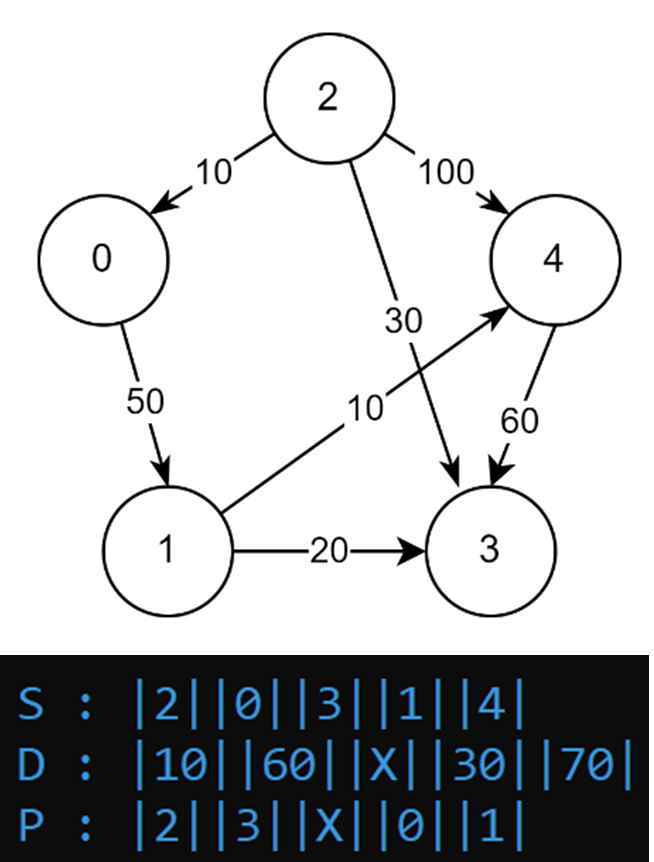
\includegraphics{imagenes/Imagen2.png}
        \caption{Ejemplo 2 del algoritmo de Dijkstra}
    \end{figure}
    El tercer grafo implementado tiene $|$V$|$=6 entonces, si se escoge como variable inicial=0 se tiene los siguientes resultados, v\'ease Figura 6.
    \begin{figure}[H]
        \centering
        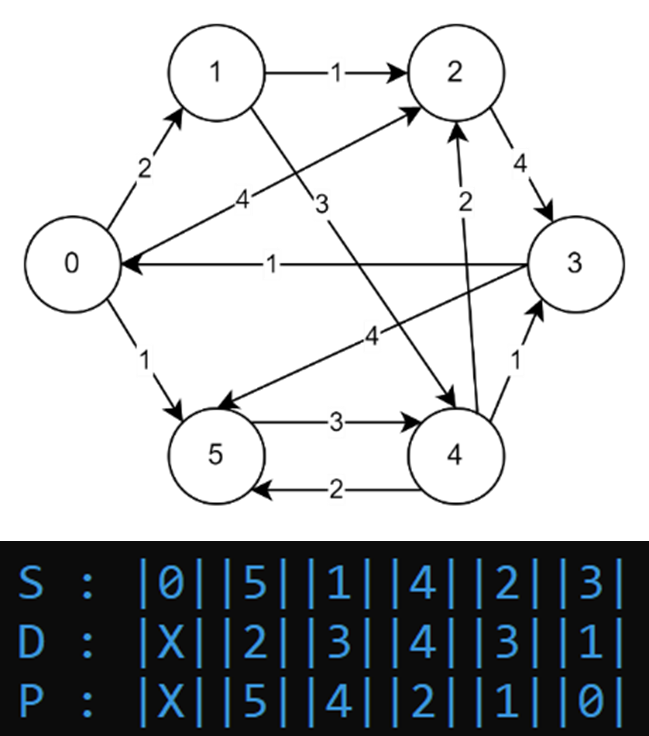
\includegraphics{imagenes/Imagen3.png}
        \caption{Ejemplo 3 del algoritmo de Dijkstra}
    \end{figure}
    El cuarto grafo implementado tiene $|$V$|$=7 entonces, si se escoge como variable inicial=2 se tiene los siguientes resultados, v\'ease Figura 7.
    \begin{figure}[H]
        \centering
        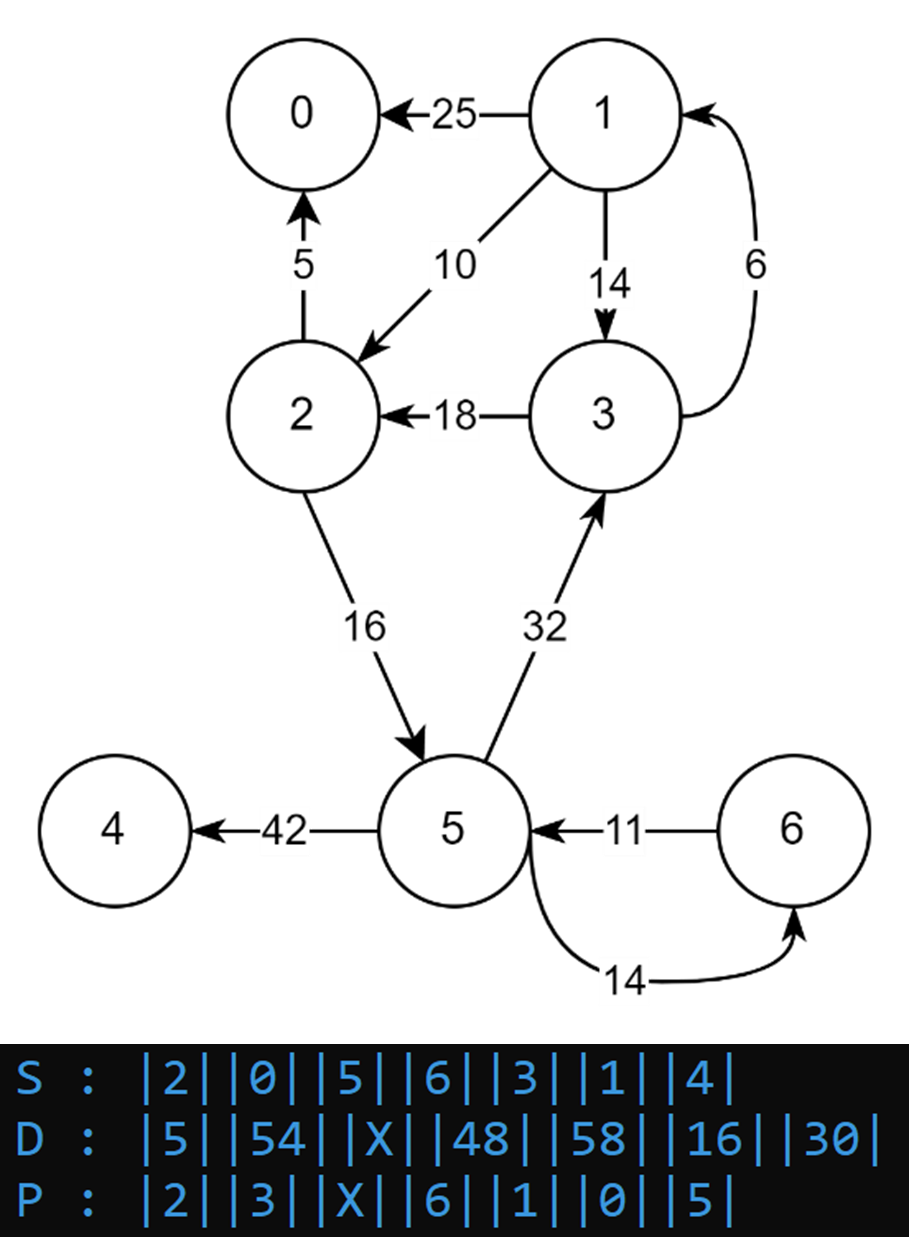
\includegraphics{imagenes/Imagen4.png}
        \caption{Ejemplo 4 del algoritmo de Dijkstra}
    \end{figure}
    El quinto grafo implementado tiene $|$V$|$=8 entonces, si se escoge como variable inicial=0 se tiene los siguientes resultados, v\'ease Figura 8.
    \begin{figure}[H]
        \centering
        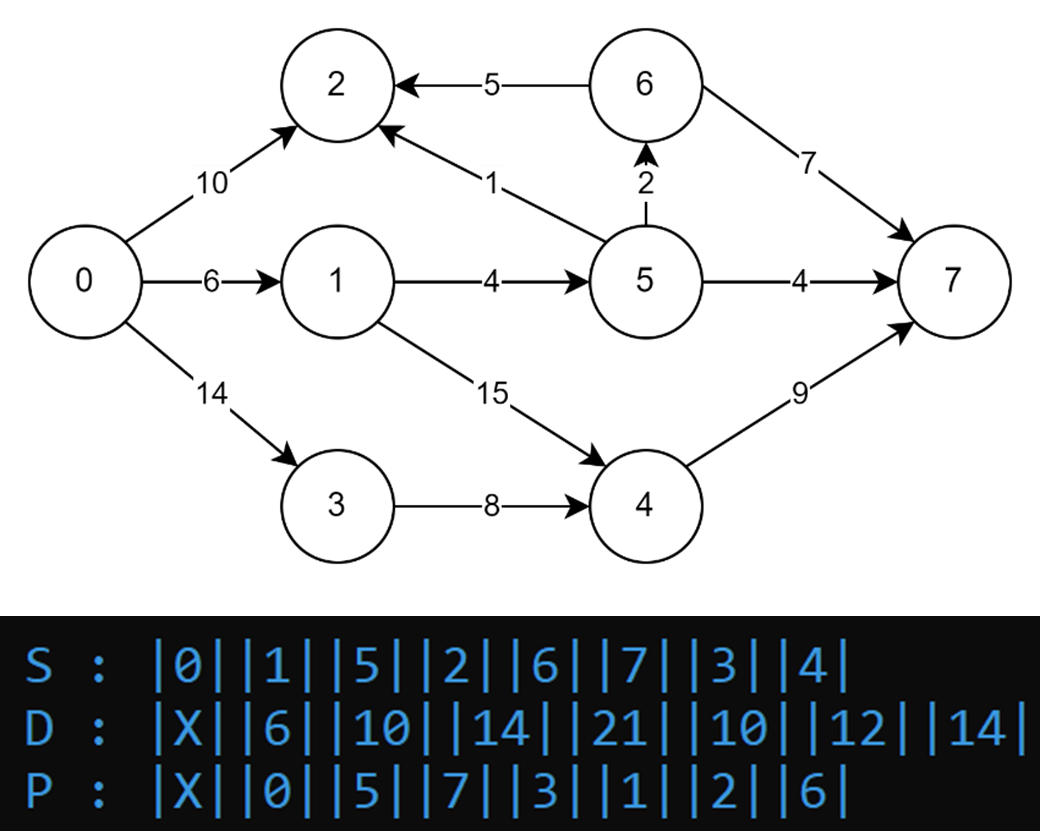
\includegraphics{imagenes/Imagen5.png}
        \caption{Ejemplo 5 del algoritmo de Dijkstra}
    \end{figure}
    El sexto grafo implementado tiene $|$V$|$=9 entonces, si se escoge como variable inicial=0 se tiene los siguientes resultados, v\'ease Figura 9.
    \begin{figure}[H]
        \centering
        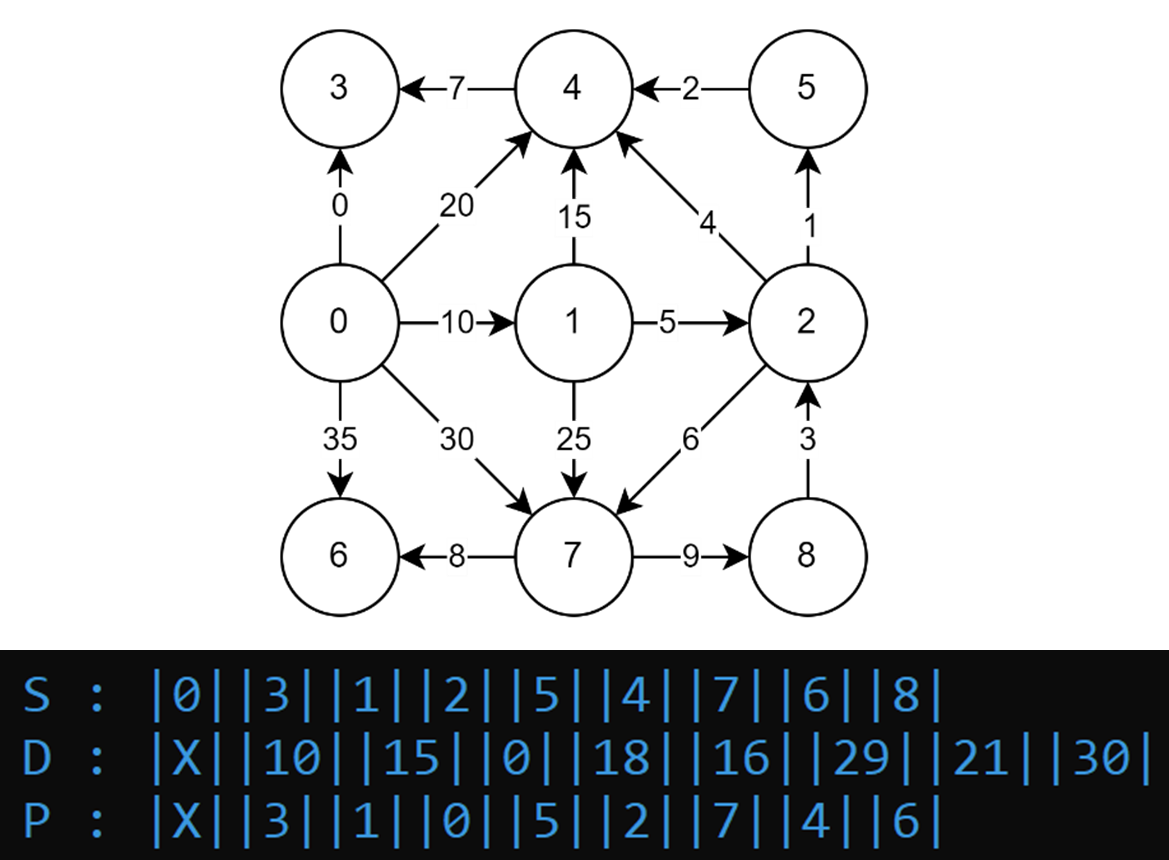
\includegraphics{imagenes/Imagen6.png}
        \caption{Ejemplo 6 del algoritmo de Dijkstra}
    \end{figure}
    Ya que el dato de entrada es un n\'umero natural (incluido el 0) $n$ que es la $|V|$,  se tiene que la salida del programa da el n\'umero de operaciones hechas por cada iteraci\'on, los resultados registrados se muestran en la Tabla 1.
    \begin{longtable}{||c|c||}
        \caption{Complejidad temporal del algoritmo de Dijkstra}\\
            \hline
                \textbf{n}&\textbf{T(n)}\\
            \hline
                {0}&{13}\\
            \hline
                {1}&{16}\\
            \hline
                {2}&{28}\\
            \hline
                {3}&{45}\\
            \hline
                {4}&{67}\\
            \hline
                {5}&{96}\\
            \hline
                {6}&{129}\\
            \hline
                {7}&{167}\\
            \hline
                {8}&{209}\\
            \hline
                {9}&{262}\\
            \hline
    \end{longtable}
    Dado el comportamiento de los puntos de muestra, se aprecia que este es cuadr\'atico, no habiendo diferencia entre el mejor y peor caso, y conociendo que $\Theta$ se define como:
    $$\Theta(g(n)) = \{ f(n)~\arrowvert~\exists_{n}~C_{1},~C_{2}>0~\&~n_{0}>0~tal~que$$ $$0\leq~C_{1}g(n)~\leq~f(n)~\leq~C_{2}g(n)~\forall~n\geq~n_{0}\}$$
    \\
    Se propone $C_{1}=\frac{20}{7}$, $C_{2}=\frac{17}{4}$ y $n_{0}=4$, es posible obsevar en la Figura 10 que dados estos valores se acotan la parte superior como la inferior as\'i como el punto de cruce en el que se cumple la inecuaci\'on, por tanto se puede decir que $T(n)\in \Theta(n^{2})$.
    \begin{figure}[H]
        \centering
        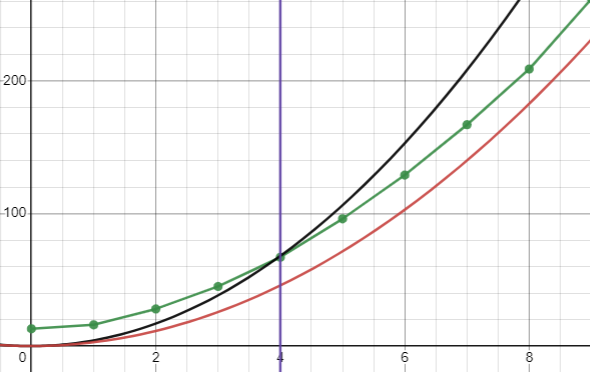
\includegraphics[width=11cm]{imagenes/p1.png}
        \caption{Gr\'afica del orden de complejidad del algoritmo de Dijkstra}
    \end{figure}
    \section{Conclusiones}
    \textbf{\large Luis Francisco Renteria Cedillo}
    \begin{figure}[H]
        \centering
        
\includegraphics[angle=0, scale=0.5]{imagenes/foto1.png}
    \end{figure}
    La importancia de obtener el camino más corto reside en alcanzar una ruta de punto A a punto B en el menor costo posible. El Algoritmo de Djikstra contribuye a solucionar este tipo de problemas en múltiples campos como la telemática, inteligencia artificial y logística para transportes. Gracias a este algoritmo se es posible resolver grafos con múltiples nodos, donde se observa lo importante y crucial que son los algoritmos Greedy.\\
    
    
    \textbf{\large Denzel Omar Vazquez Perez}
    \begin{figure}[H]
        \centering
        
\includegraphics[angle=-90, scale= 0.05]{imagenes/foto2.jpg}
    \end{figure}
    En la pr\'actica se pudo analizar el algoritmo de Dijkstra por medio de    matrices de adyacencia, donde se muestra las ventajas de usar una estrategia de programaci\'on Greedy y es que este algoritmo es muy similar al algoritmo de Prim, dado que en cada iteración, se agrega exactamente un v\'ertice al arreglo solici\'on, donde haciendo el seguimiento de la mejor ruta vista hasta la fecha para todos los vértices fuera de S y se agrega en orden de costo creciente. La diferencia entre los algoritmos de Dijkstra y Prim es cómo califican la conveniencia de cada v\'ertice.\\
    
    Finalmente, es posible decir que Dijkstra funciona bien como un algoritmo de b\'usqueda de rutas para un conjunto completo de nodos pero, cuando se usa para buscar la ruta m\'as corta a un v\'ertice específico, puede ser ineficiente, por lo que no se obtendr\'a una soluci\'on \'optima al problema en las primeras iteraciones, ya que algoritmo sigue siempre el camino con menor costo de V-S.

\section{Bibliograf\'ia}
\textsc{Busato, F., \& Bombieri, N.} (2017).\textit{Graph algorithms on GPUs. Advances in GPU Research and Practice}(pp.163–198).\\\\
\textsc{Brassard, G. (1997)}. \textit {Fundamentos de Algoritmia}. España: Ed. Prentice Hall.\\\\
\textsc{Cormen, E. A}. (2022). \textit{Introduction To Algorithms}, 3Rd Ed. Phi.\\\\
\textsc{Huang, C.-Y. (Ric), Lai, C.-Y., \& Cheng, K.-T. (Tim).} (2009).\textit{Fundamentals of algorithms. Electronic Design Automation}(pp.173–234).





\medskip

\end{document}